\documentclass[10pt]{beamer}
\usepackage[english]{babel}
\usepackage[latin1]{inputenc}
\usepackage[T1]{fontenc}
\usepackage{graphicx}
\usetheme{Montpellier}
\useoutertheme{infolines}
\usepackage{dsfont}
\usepackage{enumerate}
\usepackage{amssymb}
\usepackage{amsmath}
\usepackage{amsfonts}
\usepackage{bbm}
\usepackage[labelformat=empty]{caption}

\title{Statistics}
\author[marcio.diniz@cshs.org]{Marcio Augusto Diniz}

\date[\today]
{Biostatistics Research Center\\
Samuel Oschin Comprehensive Cancer Institute\\
Cedars Sinai Medical Center}

\AtBeginSection[]
{
  \begin{frame}<beamer>
    \frametitle{Summary}
    \tableofcontents[currentsection]
  \end{frame}
}

\begin{document}

\maketitle

\section{What is statistics?}

\subsection{History}

\begin{frame}
\frametitle{History}
\framesubtitle{}
\begin{block}{What is the origin of the word?}
\begin{itemize}
\item<1-> Statistics  is derived from the New Latin statisticum collegium (council of state) and the Italian word statista (statesman or politician);
\item<1-> The German word Statistik, first introduced by Gottfried Achenwall (1749), originally designated the systematic collection of demographic and economic data by states, signifying the science of state (then called political arithmetic in English); 
\item<2-> Tabulations of human and material resources to be taxed or put to military use.
\end{itemize}
\end{block}
\end{frame}

\begin{frame}
\frametitle{History}
\framesubtitle{}
\begin{block}{Origins}
\begin{itemize}
\item<1-> The earliest writing on statistics was found in a 9th-century book entitled: "Manuscript on Deciphering Cryptographic Messages", written by Al-Kindi (801-873 CE), describing how to use statistics and frequency analysis to decipher encrypted messages. 
\item<2-> It is often dated to 1662,  William Petty developed early human statistical and census methods that provided a framework for modern demography. He produced the first life table, giving probabilities of survival to each age, and estimated the population of London. 
\end{itemize}
\end{block}
\end{frame}

\begin{frame}
\frametitle{History}
\framesubtitle{}
\begin{block}{Games of chance}
\begin{itemize}
\item<1-> In the 16th century, Gerolamo Cardano, Pierre de Fermat and Blaise Pascal exchanged letters discussing games of chance.  Jakob Bernoulli's Ars Conjectandi (posthumous, 1713) and Abraham de Moivre's The Doctrine of Chances (1718) treated the subject as a branch of mathematics. 
\end{itemize}
\end{block}
\begin{block}{The meeting of two worlds}
\begin{itemize}
\item<1-> Adrien-Marie Legendre (1805), Robert Adrain (1808), and Carl Friedrich Gauss (1809) used probability and statistics to estimate the position of planets. 
\end{itemize}
\end{block}
\end{frame}

\begin{frame}
\frametitle{History}
\framesubtitle{}
\begin{block}{Fundamentals of Modern Statistics}
\begin{itemize}
\item<1-> At the end of 19th century, Francis Galton and Karl Pearson transformed statistics into a rigorous mathematical discipline used for analysis, not just in science;
\item<2-> In the 1910s and 20s, William Sealy Gosset and Ronald Fisher developed better design of experiments, significance tests and other methods for small sample sizes;
\item<3-> In the 1930s, Egon Pearson and Jerzy Neyman introduced the concepts of confidence intervals, test of hypothesis and power.
\end{itemize}
\end{block}
\end{frame}

\begin{frame}
\frametitle{History}
\begin{figure}[!htb]
    \centering
    \begin{minipage}{.5\textwidth}
        \centering
        \includegraphics[scale = 0.35]{book01}
        \label{fig:prob1_6_2}
    \end{minipage}%
    \begin{minipage}{0.5\textwidth}
        \centering
        \includegraphics[scale = 0.35]{book02}
        \label{fig:prob1_6_1}
    \end{minipage}
\end{figure}
\end{frame}

\subsection{Statistical Thinking}

\begin{frame}
\frametitle{Which lake does have more fishes?}
\begin{columns}
\begin{column}{0.45\textwidth}
\begin{figure}
	\centering
		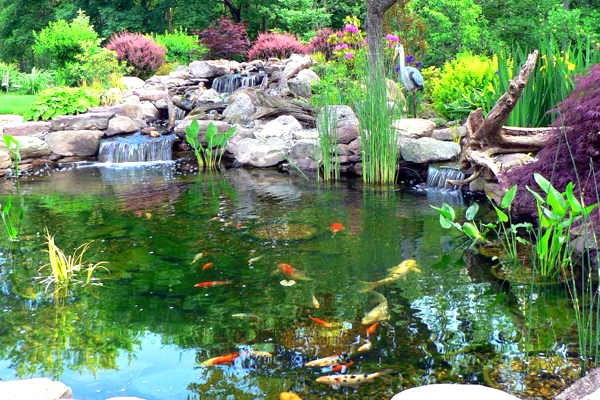
\includegraphics[scale = 0.2]{pond01.png}
	\caption{234 fishes}
	\label{fig:pond01}
\end{figure}
\end{column}
\begin{column}{0.45\textwidth}
\begin{figure}
	\centering
		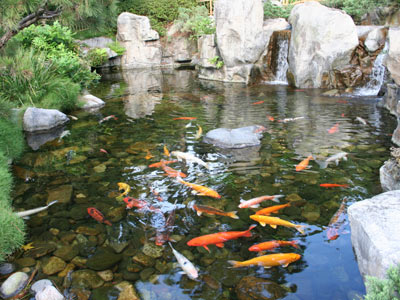
\includegraphics[scale = 0.5]{pond02.png}
	\caption{235 fishes}
	\label{fig:pond02}
\end{figure}
\end{column}
\end{columns}
\end{frame}


\begin{frame}
\frametitle{Which lake does have more fishes?}
\begin{figure}
	\centering
		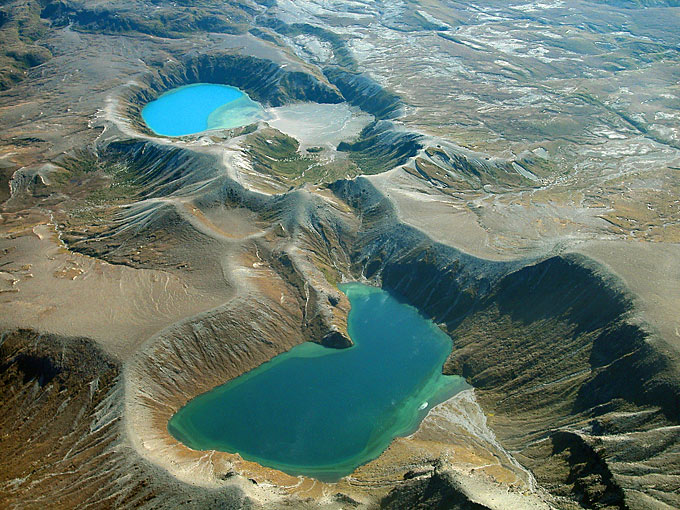
\includegraphics[scale = 0.5]{lake.png}
	\caption{234 and 235 fishes sampled}
	\label{fig:lake}
\end{figure}
\end{frame}


\begin{frame}
\frametitle{Which lake does have more fishes?}
\begin{itemize}
\item<1-> What is the difference between the first and second scenarios?
\begin{itemize}
\item<2-> In the first scenario, the total number of fishes is derived from a census, while it is from a sample in the second scenario.
\end{itemize}
\item<3-> What is the difference between census and sample?
\begin{itemize}
\item<4-> Uncertainty.
\end{itemize}
\item<5-> How do we handle uncertainty?
\begin{itemize}
\item<6-> Identify sources of variability;
\item<7-> Minimize;
\item<8-> Measure;
\item<9-> Make decisions.
\end{itemize}
\end{itemize}
\end{frame}


\begin{frame}
\frametitle{What is Statistics?}
\begin{itemize}
\item American Statistical Association, funded in 1839: It is the science of learning from data, and of measuring, controlling and communicating uncertainty.
\begin{itemize}
\item It is a \textbf{science}, therefore, statistical tools are invented and improved by statisticians over time;
\item It measures \textbf{uncertainty} allowing us to make inferences from a sample to a population.
\end{itemize}
\end{itemize}
\end{frame}

\begin{frame}
\frametitle{Which questions can we answer with statistics?}
\begin{itemize}
\item<1-> Does the new medication have any effect on tumor growth?
\item<2-> Is the treatment effect different in WT and PR-364 mouse model?
\item<3-> Which genes are differently expressed between healthy and cancer patients?
\item<4-> What is the minimum effective dose of a drug combination to give to mice aiming to increase cancer survival?
\item<5-> What is the normal range for a biomarker? 
\item<6-> Is the new biomarker useful to detect early stage cancer?
\item<7-> Which patients' baseline characteristics can predict disease free survival at 5 years?
\end{itemize}
\end{frame}

\begin{frame}
\frametitle{When should we talk to a statistician?}
\begin{figure}
	\centering
		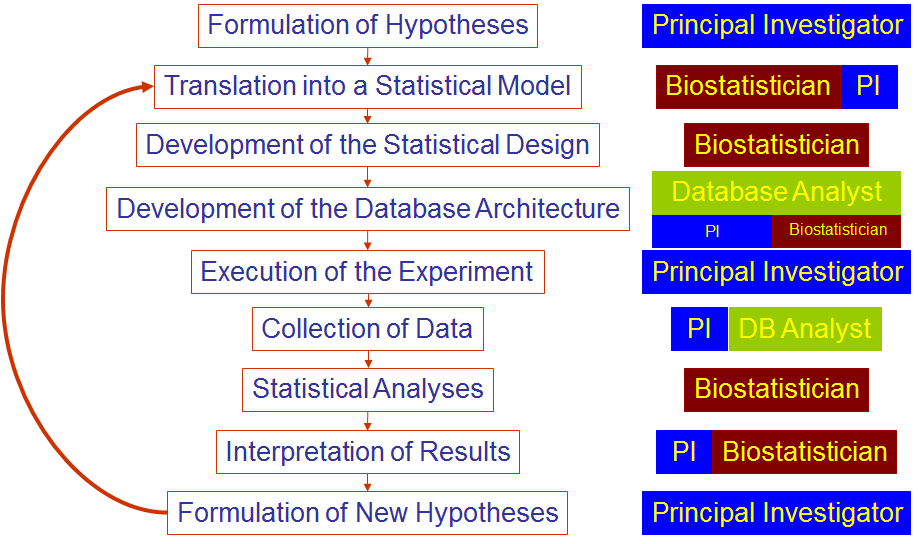
\includegraphics[scale = 0.45]{steps.png}
	\caption{Steps of Research}
	\label{fig:steps}
\end{figure}
\end{frame}

\begin{frame}
\frametitle{Cedars Sinai Medical Center}
\begin{block}{Biostatistics Core}
\begin{itemize}
\item Request Form: \url{http://www.cedars-sinai.edu/forms/cancercenter/biostatrequest.asp}
\end{itemize}
\end{block}
\begin{block}{Members}
\begin{itemize}
\item \url{http://cedars-sinai.edu/Research/Research-Cores/Biostatistical-Sciences/Staff.aspx}
\item Marcio Diniz (marcio.diniz@cshs.org)
\item Michael Luu (michael.luu@cshs.org)
\end{itemize}
\end{block}
\end{frame}

\end{document}